\pdfminorversion=6 % this is needed to be able to include pdf 1.6. 
                    % For some reasons some old HPSG proceedings have pdf 1.6
\documentclass[11pt,a4paper,fleqn]{article}
\usepackage{times}
\thispagestyle{empty}



\usepackage[T1]{fontenc}   % Silbentrennung

\usepackage[utf8x]{inputenc}
                                                                                                                             
\hyphenation{Acad-e-my}

\usepackage[bookmarks=true,bookmarksopen=true,%
breaklinks=true,%
draft=false,plainpages=false,hyperfootnotes=false,%
pdfauthor={Stefan Müller (Editor)},%
pdftitle={Proceedings of the 14th International Conference on Head-Driven Phrase Structure Grammar},%
pdfkeywords={HPSG}%,
pdftex=true%
%ps2pdf=true  %ohne diesen Treiber geht der Zeilenumbruch in URLs
]{hyperref}% for pdf files
\hypersetup{colorlinks=false, pdfborder={0 0 0}}

\usepackage{pdfpages}
\pdfinclusioncopyfonts=1

\newcommand\formatauthor[2]{\begin{tabular}[t]{@{}c@{}}
  {\LARGE#1\strut}\\
  {\small#2\strut}\\
  \rule{\dimexpr0.5\linewidth-1em}{0pt}
  \end{tabular}\xhfill\ignorespaces}
\newcommand\xhfill{\hspace{1em plus 1fill}}

\begin{document}

\begin{center}
{\Large
                {\bfseries Proceedings of the 14th International Conference on\par Head-Driven Phrase Structure Grammar\par}

                \vspace{8ex}

                     Stanford Department of Linguistics and CSLI's LinGO Lab\\[\baselineskip]

                        Stefan M{\"u}ller (Editor)\\[\baselineskip]

                                2007\\[\baselineskip]

                          CSLI Publications\\[\baselineskip]

              http://csli-publications.stanford.edu/HPSG/2007 \\[4\baselineskip]

The papers are published under a \href{http://creativecommons.org/licenses/by/4.0/}{CC-BY license}:\\[3pt]
\href{http://creativecommons.org/licenses/by/4.0/}{http://creativecommons.org/licenses/by/4.0/}
}
\end{center}
\newpage
\tableofcontents

\newpage

\section{Editor's Note}
%% -*- coding:utf-8 -*-
The 14th International Conference on Head-Driven Phrase Structure Grammar (2007) was held in Stanford
and organized by the Stanford Department of Linguistics and CSLI's LinGO Lab.

The conference featured 2 invited talks and 18 papers
selected by the program committee 
(Doug Arnold,      
Emily M. Bender,	
Olivier Bonami,	
Ann Copestake,	
Berthold Crysmann,
Dan Flickinger,	
Tibor Kiss,	
Jong-Bok Kim,	
Robert Levine,	
Tsuneko Nakazawa,
Stefan Müller (chair),
Gerald Penn,	
Adam Przepiorkowski,
Ivan Sag,	
Jesse Tseng,	
Detmar Meurers,	  
Frank Van Eynde,
Gertjan van Noord,
Gert Webelhuth,	
Stephen Wechsler).

A workshop about \emph{Constructions and Grammatical Theory}
was attached to the conference. It featured three invited talks
and 4 papers, selected by the program committee.

In total there were 38 submissions to the main conference and to the
workshop. 
We want to thank the respective program committee for putting this nice program together.



Thanks go to Ivan Sag, who was in charge of local arrangements.


As in the past years the contributions to the conference proceedings are based on the five page abstract
that was reviewed by the respective program committees, but there is no additional reviewing of the
longer contribution to the proceedings.
To ensure easy access and fast publication we have chosen an electronic format.


The proceedings include all the papers except those by Adele Goldberg and Christopher Manning.


\newpage
\part{Contributions to the Main Conference}
\thispagestyle{empty}
\newpage
        \setcounter{page}{6}
        \phantomsection
        \addcontentsline{toc}{section}{Anne Bjerre, Tavs Bjerre: Pseudocoordination in Danish}
\thispagestyle{empty}

\begin{center}
  {\huge\bfseries Pseudocoordination in Danish\par}

  \bigskip

~\\
\begingroup
\setlength{\leftskip}{0pt plus 1fill}
\setlength{\rightskip}{0pt plus 1fill}
\setlength{\parindent}{0pt}
\setlength{\parfillskip}{0pt}
  \formatauthor{Anne Bjerre}{\begin{tabular}{@{}c@{}}University of Southern Denmark\end{tabular}}
\formatauthor{Tavs Bjerre}{\begin{tabular}{@{}c@{}}Aarhus University, Denmark\end{tabular}}

\par\endgroup

  \vspace*{8ex}

  Proceedings of the 14th International Conference on\par Head-Driven Phrase Structure Grammar

  \bigskip

  Stanford Department of Linguistics and CSLI's LinGO Lab

  \medskip

  Stefan Müller (Editor)

  \medskip

  2007

  \medskip

  CSLI Publications

  \medskip

  pages 6--24

  \medskip

  \url{http://csli-publications.stanford.edu/HPSG/2007}
\end{center}
\vfill

\noindent



\vfill
\noindent
% APA Style
Bjerre, Anne, \& Bjerre,  Tavs. 2007. Pseudocoordination in Danish. In Müller, Stefan (Ed.), \emph{{Proceedings of the 14th International Conference on Head-Driven Phrase Structure Grammar, Stanford Department of Linguistics and CSLI's LinGO Lab}}, 6--24. Stanford,
CA: CSLI Publications. \hfill\href{http://creativecommons.org/licenses/by/4.0/}{\includegraphics[height=.75em]{Includes/ccby.eps}}

\newpage
\includepdf[pages=-,pagecommand=\thispagestyle{plain}]{Includes/bjerre-bjerre.pdf}
        \setcounter{page}{25}
        \phantomsection
        \addcontentsline{toc}{section}{Olivier Bonami, Dani\`{e}le Godard: Integrating Linguistic Dimensions:\\ The Scope of Adverbs}
\thispagestyle{empty}

\begin{center}
  {\huge\bfseries Integrating Linguistic Dimensions:\par The Scope of Adverbs\par}

  \bigskip

~\\
\begingroup
\setlength{\leftskip}{0pt plus 1fill}
\setlength{\rightskip}{0pt plus 1fill}
\setlength{\parindent}{0pt}
\setlength{\parfillskip}{0pt}
  \formatauthor{Olivier Bonami}{\begin{tabular}{@{}c@{}}Université Paris-Sorbonne\end{tabular}}
\formatauthor{Danièle Godard}{\begin{tabular}{@{}c@{}}LLF\end{tabular}}

\par\endgroup

  \vspace*{8ex}

  Proceedings of the 14th International Conference on\par Head-Driven Phrase Structure Grammar

  \bigskip

  Stanford Department of Linguistics and CSLI's LinGO Lab

  \medskip

  Stefan Müller (Editor)

  \medskip

  2007

  \medskip

  CSLI Publications

  \medskip

  pages 25--45

  \medskip

  \url{http://csli-publications.stanford.edu/HPSG/2007}
\end{center}
\vfill

\noindent



\vfill
\noindent
% APA Style
Bonami, Olivier, \& Godard,  Danièle. 2007. Integrating Linguistic Dimensions:  The Scope of Adverbs. In Müller, Stefan (Ed.), \emph{{Proceedings of the 14th International Conference on Head-Driven Phrase Structure Grammar, Stanford Department of Linguistics and CSLI's LinGO Lab}}, 25--45. Stanford,
CA: CSLI Publications. \hfill\href{http://creativecommons.org/licenses/by/4.0/}{\includegraphics[height=.75em]{Includes/ccby.eps}}

\newpage
\includepdf[pages=-,pagecommand=\thispagestyle{plain}]{Includes/bonami-godard.pdf}
        \setcounter{page}{46}
        \phantomsection
        \addcontentsline{toc}{section}{Rui P. Chaves, Denis Paperno: On The Russian Hybrid Coordination Construction}
\thispagestyle{empty}

\begin{center}
  {\huge\bfseries On The Russian Hybrid Coordination Construction\par}

  \bigskip

~\\
\begingroup
\setlength{\leftskip}{0pt plus 1fill}
\setlength{\rightskip}{0pt plus 1fill}
\setlength{\parindent}{0pt}
\setlength{\parfillskip}{0pt}
  \formatauthor{Rui P. Chaves}{\begin{tabular}{@{}c@{}}University of Lisbon\end{tabular}}
\formatauthor{Denis Paperno}{\begin{tabular}{@{}c@{}}Lomonosov Moscow State University\end{tabular}}

\par\endgroup

  \vspace*{8ex}

  Proceedings of the 14th International Conference on\par Head-Driven Phrase Structure Grammar

  \bigskip

  Stanford Department of Linguistics and CSLI's LinGO Lab

  \medskip

  Stefan Müller (Editor)

  \medskip

  2007

  \medskip

  CSLI Publications

  \medskip

  pages 46--64

  \medskip

  \url{http://csli-publications.stanford.edu/HPSG/2007}
\end{center}
\vfill

\noindent



\vfill
\noindent
% APA Style
Chaves, Rui P., \& Paperno, Denis. 2007. On The Russian Hybrid Coordination Construction. In Müller, Stefan (Ed.), \emph{{Proceedings of the 14th International Conference on Head-Driven Phrase Structure Grammar, Stanford Department of Linguistics and CSLI's LinGO Lab}}, 46--64. Stanford,
CA: CSLI Publications. \hfill\href{http://creativecommons.org/licenses/by/4.0/}{\includegraphics[height=.75em]{Includes/ccby.eps}}

\newpage
\includepdf[pages=-,pagecommand=\thispagestyle{plain}]{Includes/chaves-paperno.pdf}
        \setcounter{page}{65}
        \phantomsection
        \addcontentsline{toc}{section}{Lori Coulter: A Semantic Interpretation of Modality in Counterfactual Conditionals}
\thispagestyle{empty}

\begin{center}
  {\huge\bfseries A Semantic Interpretation of Modality in Counterfactual Conditionals\par}

  \bigskip

~\\
\begingroup
\setlength{\leftskip}{0pt plus 1fill}
\setlength{\rightskip}{0pt plus 1fill}
\setlength{\parindent}{0pt}
\setlength{\parfillskip}{0pt}
  \formatauthor{Lori Coulter}{\begin{tabular}{@{}c@{}}University of Illinois at Urbana Champaign\end{tabular}}

\par\endgroup

  \vspace*{8ex}

  Proceedings of the 14th International Conference on\par Head-Driven Phrase Structure Grammar

  \bigskip

  Stanford Department of Linguistics and CSLI's LinGO Lab

  \medskip

  Stefan Müller (Editor)

  \medskip

  2007

  \medskip

  CSLI Publications

  \medskip

  pages 65--82

  \medskip

  \url{http://csli-publications.stanford.edu/HPSG/2007}
\end{center}
\vfill

\noindent



\vfill
\noindent
% APA Style
Coulter, Lori. 2007. A Semantic Interpretation of Modality in Counterfactual Conditionals. In Müller, Stefan (Ed.), \emph{{Proceedings of the 14th International Conference on Head-Driven Phrase Structure Grammar, Stanford Department of Linguistics and CSLI's LinGO Lab}}, 65--82. Stanford,
CA: CSLI Publications. \hfill\href{http://creativecommons.org/licenses/by/4.0/}{\includegraphics[height=.75em]{Includes/ccby.eps}}

\newpage
\includepdf[pages=-,pagecommand=\thispagestyle{plain}]{Includes/coulter.pdf}
        \setcounter{page}{83}
        \phantomsection
        \addcontentsline{toc}{section}{Berthold Crysmann, Philipp von B{\"o}selager: Using an HPSG Grammar for the Generation of Prosody}
\thispagestyle{empty}

\begin{center}
  {\huge\bfseries Using an HPSG Grammar for the Generation of Prosody\par}

  \bigskip

~\\
\begingroup
\setlength{\leftskip}{0pt plus 1fill}
\setlength{\rightskip}{0pt plus 1fill}
\setlength{\parindent}{0pt}
\setlength{\parfillskip}{0pt}
  \formatauthor{Berthold Crysmann}{\begin{tabular}{@{}c@{}}DFKI, Universität des Saarlandes, Universität Bonn\end{tabular}}
\formatauthor{Philipp von Böselager}{\begin{tabular}{@{}c@{}}Universität zu Köln\end{tabular}}

\par\endgroup

  \vspace*{8ex}

  Proceedings of the 14th International Conference on\par Head-Driven Phrase Structure Grammar

  \bigskip

  Stanford Department of Linguistics and CSLI's LinGO Lab

  \medskip

  Stefan Müller (Editor)

  \medskip

  2007

  \medskip

  CSLI Publications

  \medskip

  pages 83--98

  \medskip

  \url{http://csli-publications.stanford.edu/HPSG/2007}
\end{center}
\vfill

\noindent



\vfill
\noindent
% APA Style
Crysmann, Berthold, \& von Böselager, Philipp. 2007. Using an HPSG Grammar for the Generation of Prosody. In Müller, Stefan (Ed.), \emph{{Proceedings of the 14th International Conference on Head-Driven Phrase Structure Grammar, Stanford Department of Linguistics and CSLI's LinGO Lab}}, 83--98. Stanford,
CA: CSLI Publications. \hfill\href{http://creativecommons.org/licenses/by/4.0/}{\includegraphics[height=.75em]{Includes/ccby.eps}}

\newpage
\includepdf[pages=-,pagecommand=\thispagestyle{plain}]{Includes/crysmann-vonboeselager.pdf}
        \setcounter{page}{99}
        \phantomsection
        \addcontentsline{toc}{section}{Mary Esther Kropp Dakubu, Lars Hellan, Dorothee Beermann: Verb Sequencing Constraints in Ga:
Serial Verb Constructions and the Extended Verb Complex}
\thispagestyle{empty}

\begin{center}
  {\huge\bfseries Verb Sequencing Constraints in Ga:
Serial Verb Constructions and the Extended Verb Complex\par}

  \bigskip

~\\
\begingroup
\setlength{\leftskip}{0pt plus 1fill}
\setlength{\rightskip}{0pt plus 1fill}
\setlength{\parindent}{0pt}
\setlength{\parfillskip}{0pt}
  \formatauthor{Mary Esther Kropp Dakubu}{\begin{tabular}{@{}c@{}}University of Ghana\end{tabular}}
\formatauthor{Lars Hellan}{\begin{tabular}{@{}c@{}}NTNU, Trondheim\end{tabular}}
\formatauthor{Dorothee Beermann}{\begin{tabular}{@{}c@{}}NTNU, Trondheim\end{tabular}}

\par\endgroup

  \vspace*{8ex}

  Proceedings of the 14th International Conference on\par Head-Driven Phrase Structure Grammar

  \bigskip

  Stanford Department of Linguistics and CSLI's LinGO Lab

  \medskip

  Stefan Müller (Editor)

  \medskip

  2007

  \medskip

  CSLI Publications

  \medskip

  pages 99--119

  \medskip

  \url{http://csli-publications.stanford.edu/HPSG/2007}
\end{center}
\vfill

\noindent



\vfill
\noindent
% APA Style
Kropp Dakubu, Mary Esther, Hellan,  Lars, \& Beermann, Dorothee. 2007. Verb Sequencing Constraints in Ga:
Serial Verb Constructions and the Extended Verb Complex. In Müller, Stefan (Ed.), \emph{{Proceedings of the 14th International Conference on Head-Driven Phrase Structure Grammar, Stanford Department of Linguistics and CSLI's LinGO Lab}}, 99--119. Stanford,
CA: CSLI Publications. \hfill\href{http://creativecommons.org/licenses/by/4.0/}{\includegraphics[height=.75em]{Includes/ccby.eps}}

\newpage
\includepdf[pages=-,pagecommand=\thispagestyle{plain}]{Includes/khb.pdf}
        \setcounter{page}{120}
        \phantomsection
        \addcontentsline{toc}{section}{Petter Haugereid: Decomposed Phrasal Constructions}
\thispagestyle{empty}

\begin{center}
  {\huge\bfseries Decomposed Phrasal Constructions\par}

  \bigskip

~\\
\begingroup
\setlength{\leftskip}{0pt plus 1fill}
\setlength{\rightskip}{0pt plus 1fill}
\setlength{\parindent}{0pt}
\setlength{\parfillskip}{0pt}
  \formatauthor{Petter Haugereid}{\begin{tabular}{@{}c@{}}NTNU Trondheim\end{tabular}}

\par\endgroup

  \vspace*{8ex}

  Proceedings of the 14th International Conference on\par Head-Driven Phrase Structure Grammar

  \bigskip

  Stanford Department of Linguistics and CSLI's LinGO Lab

  \medskip

  Stefan Müller (Editor)

  \medskip

  2007

  \medskip

  CSLI Publications

  \medskip

  pages 120--129

  \medskip

  \url{http://csli-publications.stanford.edu/HPSG/2007}
\end{center}
\vfill

\noindent



\vfill
\noindent
% APA Style
Haugereid, Petter. 2007. Decomposed Phrasal Constructions. In Müller, Stefan (Ed.), \emph{{Proceedings of the 14th International Conference on Head-Driven Phrase Structure Grammar, Stanford Department of Linguistics and CSLI's LinGO Lab}}, 120--129. Stanford,
CA: CSLI Publications. \hfill\href{http://creativecommons.org/licenses/by/4.0/}{\includegraphics[height=.75em]{Includes/ccby.eps}}

\newpage
\includepdf[pages=-,pagecommand=\thispagestyle{plain}]{Includes/haugereid.pdf}
        \setcounter{page}{130}
        \phantomsection
        \addcontentsline{toc}{section}{Fabiola Henri, Anne Abeill{\'e}: The Syntax of Copular Constructions in Mauritian}
\thispagestyle{empty}

\begin{center}
  {\huge\bfseries The Syntax of Copular Constructions in Mauritian\par}

  \bigskip

~\\
\begingroup
\setlength{\leftskip}{0pt plus 1fill}
\setlength{\rightskip}{0pt plus 1fill}
\setlength{\parindent}{0pt}
\setlength{\parfillskip}{0pt}
  \formatauthor{Fabiola Henri}{\begin{tabular}{@{}c@{}}University Paris 7\end{tabular}}
\formatauthor{Anne Abeillé}{\begin{tabular}{@{}c@{}}University Paris 7\end{tabular}}

\par\endgroup

  \vspace*{8ex}

  Proceedings of the 14th International Conference on\par Head-Driven Phrase Structure Grammar

  \bigskip

  Stanford Department of Linguistics and CSLI's LinGO Lab

  \medskip

  Stefan Müller (Editor)

  \medskip

  2007

  \medskip

  CSLI Publications

  \medskip

  pages 130--149

  \medskip

  \url{http://csli-publications.stanford.edu/HPSG/2007}
\end{center}
\vfill

\noindent



\vfill
\noindent
% APA Style
Henri, Fabiola, \& Abeillé, Anne. 2007. The Syntax of Copular Constructions in Mauritian. In Müller, Stefan (Ed.), \emph{{Proceedings of the 14th International Conference on Head-Driven Phrase Structure Grammar, Stanford Department of Linguistics and CSLI's LinGO Lab}}, 130--149. Stanford,
CA: CSLI Publications. \hfill\href{http://creativecommons.org/licenses/by/4.0/}{\includegraphics[height=.75em]{Includes/ccby.eps}}

\newpage
\includepdf[pages=-,pagecommand=\thispagestyle{plain}]{Includes/henri-abeille.pdf}
        \setcounter{page}{150}
        \phantomsection
        \addcontentsline{toc}{section}{Tobias Kaufmann, Beat Pfister: Applying Licenser Rules to a Grammar with Continuous Constituents}
\thispagestyle{empty}

\begin{center}
  {\huge\bfseries Applying Licenser Rules to a Grammar with Continuous Constituents\par}

  \bigskip

~\\
\begingroup
\setlength{\leftskip}{0pt plus 1fill}
\setlength{\rightskip}{0pt plus 1fill}
\setlength{\parindent}{0pt}
\setlength{\parfillskip}{0pt}
  \formatauthor{Tobias Kaufmann}{\begin{tabular}{@{}c@{}}ETH Zürich\end{tabular}}
\formatauthor{Beat Pfister}{\begin{tabular}{@{}c@{}}ETH Zürich\end{tabular}}

\par\endgroup

  \vspace*{8ex}

  Proceedings of the 14th International Conference on\par Head-Driven Phrase Structure Grammar

  \bigskip

  Stanford Department of Linguistics and CSLI's LinGO Lab

  \medskip

  Stefan Müller (Editor)

  \medskip

  2007

  \medskip

  CSLI Publications

  \medskip

  pages 150--162

  \medskip

  \url{http://csli-publications.stanford.edu/HPSG/2007}
\end{center}
\vfill

\noindent



\vfill
\noindent
% APA Style
Kaufmann, Tobias, \& Pfister, Beat. 2007. Applying Licenser Rules to a Grammar with Continuous Constituents. In Müller, Stefan (Ed.), \emph{{Proceedings of the 14th International Conference on Head-Driven Phrase Structure Grammar, Stanford Department of Linguistics and CSLI's LinGO Lab}}, 150--162. Stanford,
CA: CSLI Publications. \hfill\href{http://creativecommons.org/licenses/by/4.0/}{\includegraphics[height=.75em]{Includes/ccby.eps}}

\newpage
\includepdf[pages=-,pagecommand=\thispagestyle{plain}]{Includes/kaufmann-pfister.pdf}
        \setcounter{page}{163}
        \phantomsection
        \addcontentsline{toc}{section}{Jong-Bok Kim, Jaehyung Yang: Syntax and Semantics of Korean Numeral Classifier Constructions}
\thispagestyle{empty}

\begin{center}
  {\huge\bfseries Syntax and Semantics of Korean Numeral Classifier Constructions\par}

  \bigskip

~\\
\begingroup
\setlength{\leftskip}{0pt plus 1fill}
\setlength{\rightskip}{0pt plus 1fill}
\setlength{\parindent}{0pt}
\setlength{\parfillskip}{0pt}
  \formatauthor{Jong-Bok Kim}{\begin{tabular}{@{}c@{}}Kyung Hee University\end{tabular}}
\formatauthor{Jaehyung Yang}{\begin{tabular}{@{}c@{}}Kangnam University\end{tabular}}

\par\endgroup

  \vspace*{8ex}

  Proceedings of the 14th International Conference on\par Head-Driven Phrase Structure Grammar

  \bigskip

  Stanford Department of Linguistics and CSLI's LinGO Lab

  \medskip

  Stefan Müller (Editor)

  \medskip

  2007

  \medskip

  CSLI Publications

  \medskip

  pages 163--172

  \medskip

  \url{http://csli-publications.stanford.edu/HPSG/2007}
\end{center}
\vfill

\noindent



\vfill
\noindent
% APA Style
Kim, Jong-Bok, \& Yang,  Jaehyung. 2007. Syntax and Semantics of Korean Numeral Classifier Constructions. In Müller, Stefan (Ed.), \emph{{Proceedings of the 14th International Conference on Head-Driven Phrase Structure Grammar, Stanford Department of Linguistics and CSLI's LinGO Lab}}, 163--172. Stanford,
CA: CSLI Publications. \hfill\href{http://creativecommons.org/licenses/by/4.0/}{\includegraphics[height=.75em]{Includes/ccby.eps}}

\newpage
\includepdf[pages=-,pagecommand=\thispagestyle{plain}]{Includes/kim-yang.pdf}
        \setcounter{page}{173}
        \phantomsection
        \addcontentsline{toc}{section}{Nurit Melnik: Extending Partial Pro-drop in Modern Hebrew: A Comprehensive Analysis}
\thispagestyle{empty}

\begin{center}
  {\huge\bfseries Extending Partial Pro-drop in Modern Hebrew: A Comprehensive Analysis\par}

  \bigskip

~\\
\begingroup
\setlength{\leftskip}{0pt plus 1fill}
\setlength{\rightskip}{0pt plus 1fill}
\setlength{\parindent}{0pt}
\setlength{\parfillskip}{0pt}
  \formatauthor{Nurit Melnik}{\begin{tabular}{@{}c@{}}University of Haifa\end{tabular}}

\par\endgroup

  \vspace*{8ex}

  Proceedings of the 14th International Conference on\par Head-Driven Phrase Structure Grammar

  \bigskip

  Stanford Department of Linguistics and CSLI's LinGO Lab

  \medskip

  Stefan Müller (Editor)

  \medskip

  2007

  \medskip

  CSLI Publications

  \medskip

  pages 173--193

  \medskip

  \url{http://csli-publications.stanford.edu/HPSG/2007}
\end{center}
\vfill

\noindent



\vfill
\noindent
% APA Style
Melnik, Nurit. 2007. Extending Partial Pro-drop in Modern Hebrew: A Comprehensive Analysis. In Müller, Stefan (Ed.), \emph{{Proceedings of the 14th International Conference on Head-Driven Phrase Structure Grammar, Stanford Department of Linguistics and CSLI's LinGO Lab}}, 173--193. Stanford,
CA: CSLI Publications. \hfill\href{http://creativecommons.org/licenses/by/4.0/}{\includegraphics[height=.75em]{Includes/ccby.eps}}

\newpage
\includepdf[pages=-,pagecommand=\thispagestyle{plain}]{Includes/melnik.pdf}
        \setcounter{page}{194}
        \phantomsection
        \addcontentsline{toc}{section}{Elisabeth Norcliffe: Constructing Spanish Complex Predicates}
\thispagestyle{empty}

\begin{center}
  {\huge\bfseries Constructing Spanish Complex Predicates\par}

  \bigskip

~\\
\begingroup
\setlength{\leftskip}{0pt plus 1fill}
\setlength{\rightskip}{0pt plus 1fill}
\setlength{\parindent}{0pt}
\setlength{\parfillskip}{0pt}
  \formatauthor{Elisabeth Norcliffe}{\begin{tabular}{@{}c@{}}Stanford University\end{tabular}}

\par\endgroup

  \vspace*{8ex}

  Proceedings of the 14th International Conference on\par Head-Driven Phrase Structure Grammar

  \bigskip

  Stanford Department of Linguistics and CSLI's LinGO Lab

  \medskip

  Stefan Müller (Editor)

  \medskip

  2007

  \medskip

  CSLI Publications

  \medskip

  pages 194--213

  \medskip

  \url{http://csli-publications.stanford.edu/HPSG/2007}
\end{center}
\vfill

\noindent



\vfill
\noindent
% APA Style
Norcliffe, Elisabeth. 2007. Constructing Spanish Complex Predicates. In Müller, Stefan (Ed.), \emph{{Proceedings of the 14th International Conference on Head-Driven Phrase Structure Grammar, Stanford Department of Linguistics and CSLI's LinGO Lab}}, 194--213. Stanford,
CA: CSLI Publications. \hfill\href{http://creativecommons.org/licenses/by/4.0/}{\includegraphics[height=.75em]{Includes/ccby.eps}}

\newpage
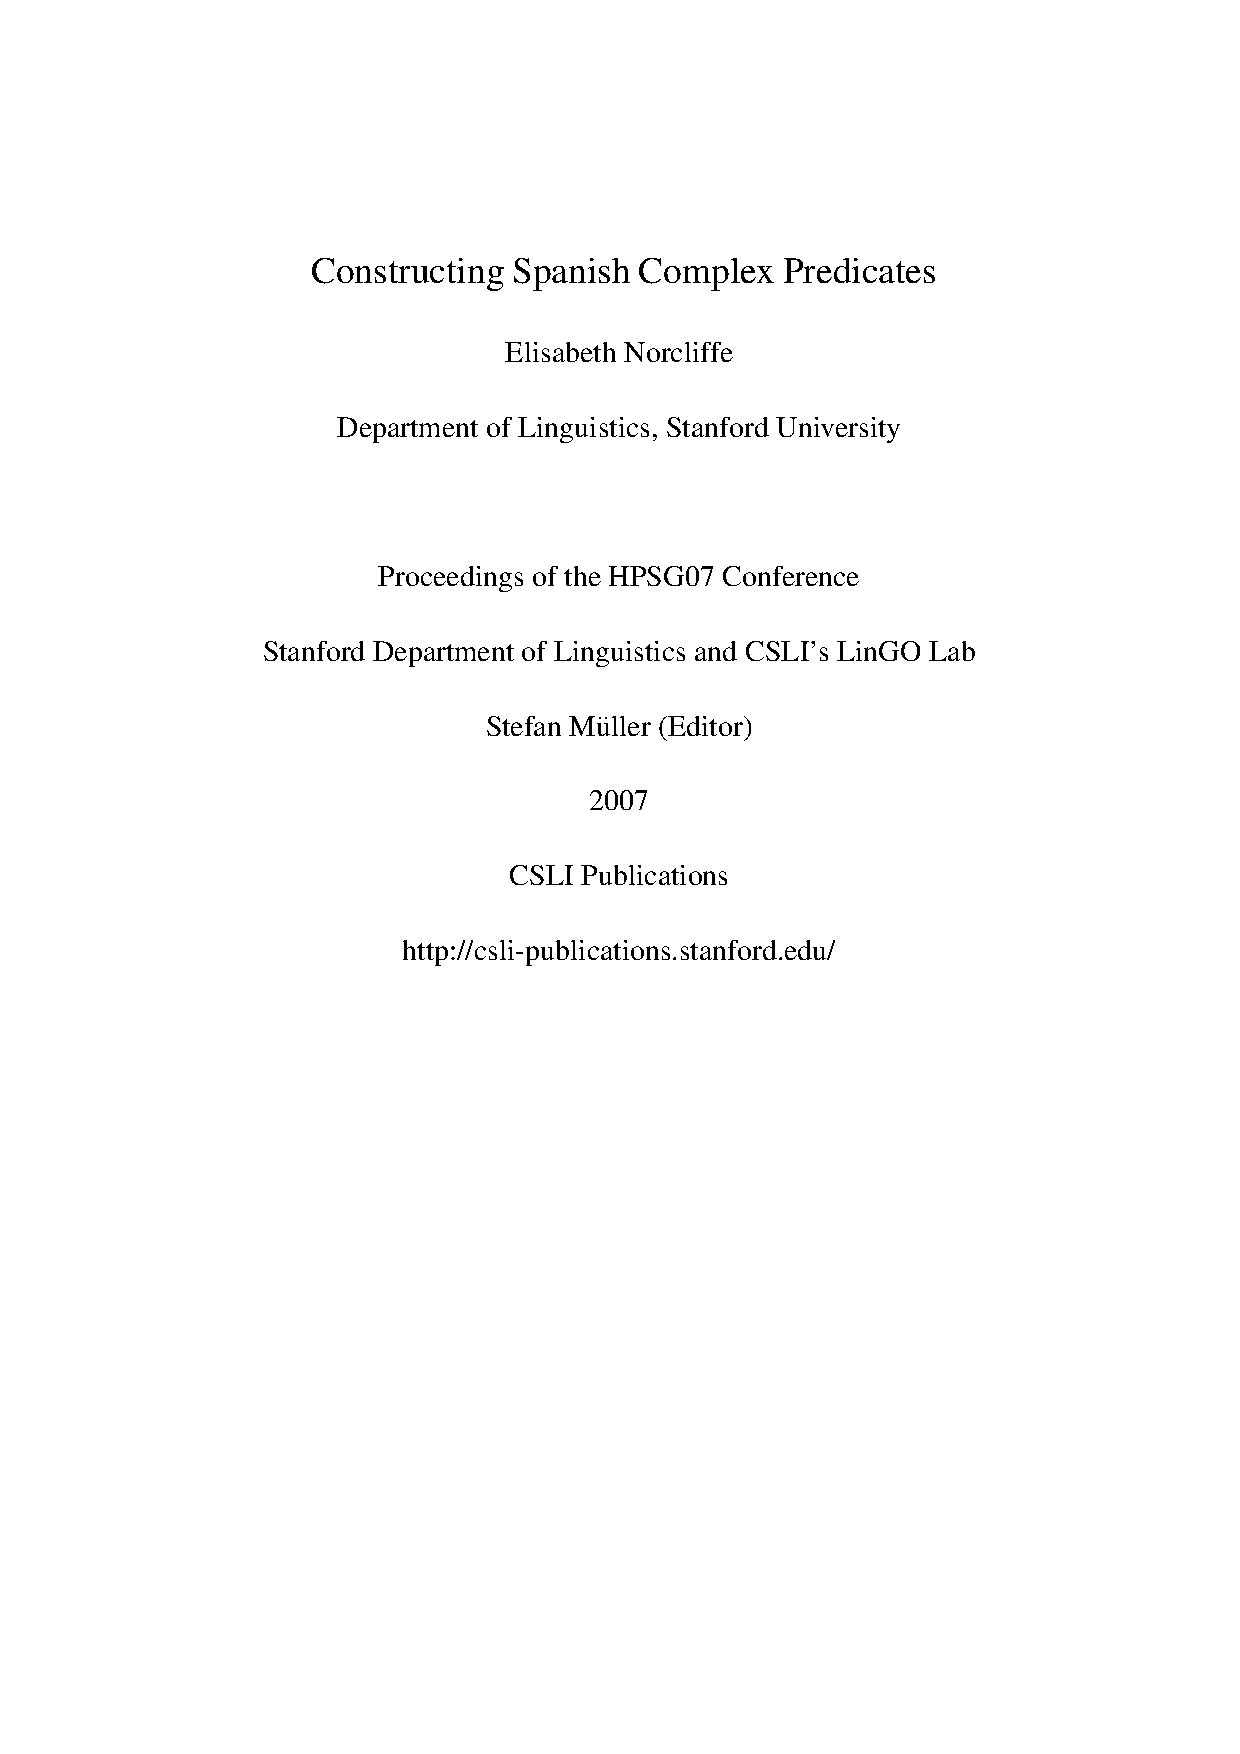
\includepdf[pages=-,pagecommand=\thispagestyle{plain}]{Includes/norcliffe.pdf}
        \setcounter{page}{214}
        \phantomsection
        \addcontentsline{toc}{section}{Manfred Sailer: NPI Licensing, Intervention and Discourse Representation Structures in HPSG}
\thispagestyle{empty}

\begin{center}
  {\huge\bfseries NPI Licensing, Intervention and Discourse Representation Structures in HPSG\par}

  \bigskip

~\\
\begingroup
\setlength{\leftskip}{0pt plus 1fill}
\setlength{\rightskip}{0pt plus 1fill}
\setlength{\parindent}{0pt}
\setlength{\parfillskip}{0pt}
  \formatauthor{Manfred Sailer}{\begin{tabular}{@{}c@{}}Universität Göttingen\end{tabular}}

\par\endgroup

  \vspace*{8ex}

  Proceedings of the 14th International Conference on\par Head-Driven Phrase Structure Grammar

  \bigskip

  Stanford Department of Linguistics and CSLI's LinGO Lab

  \medskip

  Stefan Müller (Editor)

  \medskip

  2007

  \medskip

  CSLI Publications

  \medskip

  pages 214--234

  \medskip

  \url{http://csli-publications.stanford.edu/HPSG/2007}
\end{center}
\vfill

\noindent



\vfill
\noindent
% APA Style
Sailer, Manfred. 2007. NPI Licensing, Intervention and Discourse Representation Structures in HPSG. In Müller, Stefan (Ed.), \emph{{Proceedings of the 14th International Conference on Head-Driven Phrase Structure Grammar, Stanford Department of Linguistics and CSLI's LinGO Lab}}, 214--234. Stanford,
CA: CSLI Publications. \hfill\href{http://creativecommons.org/licenses/by/4.0/}{\includegraphics[height=.75em]{Includes/ccby.eps}}

\newpage
\includepdf[pages=-,pagecommand=\thispagestyle{plain}]{Includes/sailer.pdf}
        \setcounter{page}{235}
        \phantomsection
        \addcontentsline{toc}{section}{Pollet Samvelian: A Lexical Account of Sorani Kurdish Prepositions}
\thispagestyle{empty}

\begin{center}
  {\huge\bfseries A Lexical Account of Sorani Kurdish Prepositions\par}

  \bigskip

~\\
\begingroup
\setlength{\leftskip}{0pt plus 1fill}
\setlength{\rightskip}{0pt plus 1fill}
\setlength{\parindent}{0pt}
\setlength{\parfillskip}{0pt}
  \formatauthor{Pollet Samvelian}{\begin{tabular}{@{}c@{}}Université de Paris 3\end{tabular}}

\par\endgroup

  \vspace*{8ex}

  Proceedings of the 14th International Conference on\par Head-Driven Phrase Structure Grammar

  \bigskip

  Stanford Department of Linguistics and CSLI's LinGO Lab

  \medskip

  Stefan Müller (Editor)

  \medskip

  2007

  \medskip

  CSLI Publications

  \medskip

  pages 235--249

  \medskip

  \url{http://csli-publications.stanford.edu/HPSG/2007}
\end{center}
\vfill

\noindent



\vfill
\noindent
% APA Style
Samvelian, Pollet. 2007. A Lexical Account of Sorani Kurdish Prepositions. In Müller, Stefan (Ed.), \emph{{Proceedings of the 14th International Conference on Head-Driven Phrase Structure Grammar, Stanford Department of Linguistics and CSLI's LinGO Lab}}, 235--249. Stanford,
CA: CSLI Publications. \hfill\href{http://creativecommons.org/licenses/by/4.0/}{\includegraphics[height=.75em]{Includes/ccby.eps}}

\newpage
\includepdf[pages=-,pagecommand=\thispagestyle{plain}]{Includes/samvelian.pdf}
        \setcounter{page}{250}
        \phantomsection
        \addcontentsline{toc}{section}{Sanghoun Song, Jae-Woong Choe: Type Hierarchies for Passive Forms in Korean}
\thispagestyle{empty}

\begin{center}
  {\huge\bfseries Type Hierarchies for Passive Forms in Korean\par}

  \bigskip

~\\
\begingroup
\setlength{\leftskip}{0pt plus 1fill}
\setlength{\rightskip}{0pt plus 1fill}
\setlength{\parindent}{0pt}
\setlength{\parfillskip}{0pt}
  \formatauthor{Sanghoun Song}{\begin{tabular}{@{}c@{}}Korea University\end{tabular}}
\formatauthor{Jae-Woong Choe}{\begin{tabular}{@{}c@{}}Korea University\end{tabular}}

\par\endgroup

  \vspace*{8ex}

  Proceedings of the 14th International Conference on\par Head-Driven Phrase Structure Grammar

  \bigskip

  Stanford Department of Linguistics and CSLI's LinGO Lab

  \medskip

  Stefan Müller (Editor)

  \medskip

  2007

  \medskip

  CSLI Publications

  \medskip

  pages 250--270

  \medskip

  \url{http://csli-publications.stanford.edu/HPSG/2007}
\end{center}
\vfill

\noindent



\vfill
\noindent
% APA Style
Song, Sanghoun, \& Choe, Jae-Woong. 2007. Type Hierarchies for Passive Forms in Korean. In Müller, Stefan (Ed.), \emph{{Proceedings of the 14th International Conference on Head-Driven Phrase Structure Grammar, Stanford Department of Linguistics and CSLI's LinGO Lab}}, 250--270. Stanford,
CA: CSLI Publications. \hfill\href{http://creativecommons.org/licenses/by/4.0/}{\includegraphics[height=.75em]{Includes/ccby.eps}}

\newpage
\includepdf[pages=-,pagecommand=\thispagestyle{plain}]{Includes/song-choe.pdf}
        \setcounter{page}{271}
        \phantomsection
        \addcontentsline{toc}{section}{Jesse Tseng: English Prepositional Passive Constructions}
\thispagestyle{empty}

\begin{center}
  {\huge\bfseries English Prepositional Passive Constructions\par}

  \bigskip

~\\
\begingroup
\setlength{\leftskip}{0pt plus 1fill}
\setlength{\rightskip}{0pt plus 1fill}
\setlength{\parindent}{0pt}
\setlength{\parfillskip}{0pt}
  \formatauthor{Jesse Tseng}{\begin{tabular}{@{}c@{}}CNRS\end{tabular}}

\par\endgroup

  \vspace*{8ex}

  Proceedings of the 14th International Conference on\par Head-Driven Phrase Structure Grammar

  \bigskip

  Stanford Department of Linguistics and CSLI's LinGO Lab

  \medskip

  Stefan Müller (Editor)

  \medskip

  2007

  \medskip

  CSLI Publications

  \medskip

  pages 271--286

  \medskip

  \url{http://csli-publications.stanford.edu/HPSG/2007}
\end{center}
\vfill

\noindent



\vfill
\noindent
% APA Style
Tseng, Jesse. 2007. English Prepositional Passive Constructions. In Müller, Stefan (Ed.), \emph{{Proceedings of the 14th International Conference on Head-Driven Phrase Structure Grammar, Stanford Department of Linguistics and CSLI's LinGO Lab}}, 271--286. Stanford,
CA: CSLI Publications. \hfill\href{http://creativecommons.org/licenses/by/4.0/}{\includegraphics[height=.75em]{Includes/ccby.eps}}

\newpage
\includepdf[pages=-,pagecommand=\thispagestyle{plain}]{Includes/tseng.pdf}
        \setcounter{page}{287}
        \phantomsection
        \addcontentsline{toc}{section}{Lulu Wang, Haitao Liu: A Description of Chinese NPs using Head-Driven Phrase Structure Grammar}
\thispagestyle{empty}

\begin{center}
  {\huge\bfseries A Description of Chinese NPs using Head-Driven Phrase Structure Grammar\par}

  \bigskip

~\\
\begingroup
\setlength{\leftskip}{0pt plus 1fill}
\setlength{\rightskip}{0pt plus 1fill}
\setlength{\parindent}{0pt}
\setlength{\parfillskip}{0pt}
  \formatauthor{Lulu Wang}{\begin{tabular}{@{}c@{}}Communication University of China\end{tabular}}
\formatauthor{Haitao Liu}{\begin{tabular}{@{}c@{}}Communication University of China\end{tabular}}

\par\endgroup

  \vspace*{8ex}

  Proceedings of the 14th International Conference on\par Head-Driven Phrase Structure Grammar

  \bigskip

  Stanford Department of Linguistics and CSLI's LinGO Lab

  \medskip

  Stefan Müller (Editor)

  \medskip

  2007

  \medskip

  CSLI Publications

  \medskip

  pages 287--305

  \medskip

  \url{http://csli-publications.stanford.edu/HPSG/2007}
\end{center}
\vfill

\noindent



\vfill
\noindent
% APA Style
Wang, Lulu, \& Liu, Haitao. 2007. A Description of Chinese NPs using Head-Driven Phrase Structure Grammar. In Müller, Stefan (Ed.), \emph{{Proceedings of the 14th International Conference on Head-Driven Phrase Structure Grammar, Stanford Department of Linguistics and CSLI's LinGO Lab}}, 287--305. Stanford,
CA: CSLI Publications. \hfill\href{http://creativecommons.org/licenses/by/4.0/}{\includegraphics[height=.75em]{Includes/ccby.eps}}

\newpage
\includepdf[pages=-,pagecommand=\thispagestyle{plain}]{Includes/wang-liu.pdf}
        \setcounter{page}{306}
        \phantomsection
        \addcontentsline{toc}{section}{Gert Webelhuth: Complex Topic-Comment Structures in HPSG}
\thispagestyle{empty}

\begin{center}
  {\huge\bfseries Complex Topic-Comment Structures in HPSG\par}

  \bigskip

~\\
\begingroup
\setlength{\leftskip}{0pt plus 1fill}
\setlength{\rightskip}{0pt plus 1fill}
\setlength{\parindent}{0pt}
\setlength{\parfillskip}{0pt}
  \formatauthor{Gert Webelhuth}{\begin{tabular}{@{}c@{}}University of Göttingen\end{tabular}}

\par\endgroup

  \vspace*{8ex}

  Proceedings of the 14th International Conference on\par Head-Driven Phrase Structure Grammar

  \bigskip

  Stanford Department of Linguistics and CSLI's LinGO Lab

  \medskip

  Stefan Müller (Editor)

  \medskip

  2007

  \medskip

  CSLI Publications

  \medskip

  pages 306--322

  \medskip

  \url{http://csli-publications.stanford.edu/HPSG/2007}
\end{center}
\vfill

\noindent



\vfill
\noindent
% APA Style
Webelhuth, Gert. 2007. Complex Topic-Comment Structures in HPSG. In Müller, Stefan (Ed.), \emph{{Proceedings of the 14th International Conference on Head-Driven Phrase Structure Grammar, Stanford Department of Linguistics and CSLI's LinGO Lab}}, 306--322. Stanford,
CA: CSLI Publications. \hfill\href{http://creativecommons.org/licenses/by/4.0/}{\includegraphics[height=.75em]{Includes/ccby.eps}}

\newpage
\includepdf[pages=-,pagecommand=\thispagestyle{plain}]{Includes/webelhuth.pdf}
        \setcounter{page}{323}
        \phantomsection
        \addcontentsline{toc}{section}{Sh{\^u}ichi Yatabe: Evidence for the Linearization-Based Theory of Semantic Composition}
\thispagestyle{empty}

\begin{center}
  {\huge\bfseries Evidence for the Linearization-Based Theory of Semantic Composition\par}

  \bigskip

~\\
\begingroup
\setlength{\leftskip}{0pt plus 1fill}
\setlength{\rightskip}{0pt plus 1fill}
\setlength{\parindent}{0pt}
\setlength{\parfillskip}{0pt}
  \formatauthor{Shûichi Yatabe}{\begin{tabular}{@{}c@{}}University of Tokyo\end{tabular}}

\par\endgroup

  \vspace*{8ex}

  Proceedings of the 14th International Conference on\par Head-Driven Phrase Structure Grammar

  \bigskip

  Stanford Department of Linguistics and CSLI's LinGO Lab

  \medskip

  Stefan Müller (Editor)

  \medskip

  2007

  \medskip

  CSLI Publications

  \medskip

  pages 323--343

  \medskip

  \url{http://csli-publications.stanford.edu/HPSG/2007}
\end{center}
\vfill

\noindent



\vfill
\noindent
% APA Style
Yatabe, Shûichi. 2007. Evidence for the Linearization-Based Theory of Semantic Composition. In Müller, Stefan (Ed.), \emph{{Proceedings of the 14th International Conference on Head-Driven Phrase Structure Grammar, Stanford Department of Linguistics and CSLI's LinGO Lab}}, 323--343. Stanford,
CA: CSLI Publications. \hfill\href{http://creativecommons.org/licenses/by/4.0/}{\includegraphics[height=.75em]{Includes/ccby.eps}}

\newpage
\includepdf[pages=-,pagecommand=\thispagestyle{plain}]{Includes/yatabe.pdf}
\part{Contributions to the Workshop}
\thispagestyle{empty}
\newpage
        \setcounter{page}{345}
        \phantomsection
        \addcontentsline{toc}{section}{Elaine J. Francis: The Role of Default Constructions in the Processing of Mismatch: the Case of Possessive Free Relatives}
\thispagestyle{empty}

\begin{center}
  {\huge\bfseries The Role of Default Constructions in the Processing of Mismatch: the Case of Possessive Free Relatives\par}

  \bigskip

~\\
\begingroup
\setlength{\leftskip}{0pt plus 1fill}
\setlength{\rightskip}{0pt plus 1fill}
\setlength{\parindent}{0pt}
\setlength{\parfillskip}{0pt}
  \formatauthor{Elaine J. Francis}{\begin{tabular}{@{}c@{}}Purdue University\end{tabular}}

\par\endgroup

  \vspace*{8ex}

  Proceedings of the 14th International Conference on\par Head-Driven Phrase Structure Grammar

  \bigskip

  Stanford Department of Linguistics and CSLI's LinGO Lab

  \medskip

  Stefan Müller (Editor)

  \medskip

  2007

  \medskip

  CSLI Publications

  \medskip

  pages 345--363

  \medskip

  \url{http://csli-publications.stanford.edu/HPSG/2007}
\end{center}
\vfill

\noindent



\vfill
\noindent
% APA Style
Francis, Elaine J. 2007. The Role of Default Constructions in the Processing of Mismatch: the Case of Possessive Free Relatives. In Müller, Stefan (Ed.), \emph{{Proceedings of the 14th International Conference on Head-Driven Phrase Structure Grammar, Stanford Department of Linguistics and CSLI's LinGO Lab}}, 345--363. Stanford,
CA: CSLI Publications. \hfill\href{http://creativecommons.org/licenses/by/4.0/}{\includegraphics[height=.75em]{Includes/ccby.eps}}

\newpage
\includepdf[pages=-,pagecommand=\thispagestyle{plain}]{Includes/francis.pdf}
        \setcounter{page}{364}
        \phantomsection
        \addcontentsline{toc}{section}{Jong-Bok Kim, Peter Sells: Two Types of Multiple Nominative Construction: A Constructional Approach}
\thispagestyle{empty}

\begin{center}
  {\huge\bfseries Two Types of Multiple Nominative Construction: A Constructional Approach\par}

  \bigskip

~\\
\begingroup
\setlength{\leftskip}{0pt plus 1fill}
\setlength{\rightskip}{0pt plus 1fill}
\setlength{\parindent}{0pt}
\setlength{\parfillskip}{0pt}
  \formatauthor{Jong-Bok Kim}{\begin{tabular}{@{}c@{}}Kyung Hee University\end{tabular}}
\formatauthor{Peter Sells}{\begin{tabular}{@{}c@{}}Stanford University\end{tabular}}

\par\endgroup

  \vspace*{8ex}

  Proceedings of the 14th International Conference on\par Head-Driven Phrase Structure Grammar

  \bigskip

  Stanford Department of Linguistics and CSLI's LinGO Lab

  \medskip

  Stefan Müller (Editor)

  \medskip

  2007

  \medskip

  CSLI Publications

  \medskip

  pages 364--372

  \medskip

  \url{http://csli-publications.stanford.edu/HPSG/2007}
\end{center}
\vfill

\noindent



\vfill
\noindent
% APA Style
Kim, Jong-Bok, \& Sells, Peter. 2007. Two Types of Multiple Nominative Construction: A Constructional Approach. In Müller, Stefan (Ed.), \emph{{Proceedings of the 14th International Conference on Head-Driven Phrase Structure Grammar, Stanford Department of Linguistics and CSLI's LinGO Lab}}, 364--372. Stanford,
CA: CSLI Publications. \hfill\href{http://creativecommons.org/licenses/by/4.0/}{\includegraphics[height=.75em]{Includes/ccby.eps}}

\newpage
\includepdf[pages=-,pagecommand=\thispagestyle{plain}]{Includes/kim-sells.pdf}
        \setcounter{page}{373}
        \phantomsection
        \addcontentsline{toc}{section}{Stefan M{\"u}ller: Phrasal or Lexical Constructions? Some Comments on Underspecification of Constituent Order, Compositionality, and Control}
\thispagestyle{empty}

\begin{center}
  {\huge\bfseries Phrasal or Lexical Constructions? Some Comments on Underspecification of Constituent Order, Compositionality, and Control\par}

  \bigskip

~\\
\begingroup
\setlength{\leftskip}{0pt plus 1fill}
\setlength{\rightskip}{0pt plus 1fill}
\setlength{\parindent}{0pt}
\setlength{\parfillskip}{0pt}
  \formatauthor{Stefan Müller}{\begin{tabular}{@{}c@{}}Freie Universität Berlin\end{tabular}}

\par\endgroup

  \vspace*{8ex}

  Proceedings of the 14th International Conference on\par Head-Driven Phrase Structure Grammar

  \bigskip

  Stanford Department of Linguistics and CSLI's LinGO Lab

  \medskip

  Stefan Müller (Editor)

  \medskip

  2007

  \medskip

  CSLI Publications

  \medskip

  pages 373--393

  \medskip

  \url{http://csli-publications.stanford.edu/HPSG/2007}
\end{center}
\vfill

\noindent



\vfill
\noindent
% APA Style
Müller, Stefan. 2007. Phrasal or Lexical Constructions? Some Comments on Underspecification of Constituent Order, Compositionality, and Control. In Müller, Stefan (Ed.), \emph{{Proceedings of the 14th International Conference on Head-Driven Phrase Structure Grammar, Stanford Department of Linguistics and CSLI's LinGO Lab}}, 373--393. Stanford,
CA: CSLI Publications. \hfill\href{http://creativecommons.org/licenses/by/4.0/}{\includegraphics[height=.75em]{Includes/ccby.eps}}

\newpage
\includepdf[pages=-,pagecommand=\thispagestyle{plain}]{Includes/mueller.pdf}
        \setcounter{page}{394}
        \phantomsection
        \addcontentsline{toc}{section}{Ivan A. Sag: Remarks on Locality}
\thispagestyle{empty}

\begin{center}
  {\huge\bfseries Remarks on Locality\par}

  \bigskip

~\\
\begingroup
\setlength{\leftskip}{0pt plus 1fill}
\setlength{\rightskip}{0pt plus 1fill}
\setlength{\parindent}{0pt}
\setlength{\parfillskip}{0pt}
  \formatauthor{Ivan A. Sag}{\begin{tabular}{@{}c@{}}Stanford University\end{tabular}}

\par\endgroup

  \vspace*{8ex}

  Proceedings of the 14th International Conference on\par Head-Driven Phrase Structure Grammar

  \bigskip

  Stanford Department of Linguistics and CSLI's LinGO Lab

  \medskip

  Stefan Müller (Editor)

  \medskip

  2007

  \medskip

  CSLI Publications

  \medskip

  pages 394--414

  \medskip

  \url{http://csli-publications.stanford.edu/HPSG/2007}
\end{center}
\vfill

\noindent



\vfill
\noindent
% APA Style
Sag, Ivan A. 2007. Remarks on Locality. In Müller, Stefan (Ed.), \emph{{Proceedings of the 14th International Conference on Head-Driven Phrase Structure Grammar, Stanford Department of Linguistics and CSLI's LinGO Lab}}, 394--414. Stanford,
CA: CSLI Publications. \hfill\href{http://creativecommons.org/licenses/by/4.0/}{\includegraphics[height=.75em]{Includes/ccby.eps}}

\newpage
\includepdf[pages=-,pagecommand=\thispagestyle{plain}]{Includes/sag.pdf}
        \setcounter{page}{415}
        \phantomsection
        \addcontentsline{toc}{section}{Frank Van Eynde: The Big Mess Construction}
\thispagestyle{empty}

\begin{center}
  {\huge\bfseries The Big Mess Construction\par}

  \bigskip

~\\
\begingroup
\setlength{\leftskip}{0pt plus 1fill}
\setlength{\rightskip}{0pt plus 1fill}
\setlength{\parindent}{0pt}
\setlength{\parfillskip}{0pt}
  \formatauthor{Frank Van Eynde}{\begin{tabular}{@{}c@{}}University of Leuven\end{tabular}}

\par\endgroup

  \vspace*{8ex}

  Proceedings of the 14th International Conference on\par Head-Driven Phrase Structure Grammar

  \bigskip

  Stanford Department of Linguistics and CSLI's LinGO Lab

  \medskip

  Stefan Müller (Editor)

  \medskip

  2007

  \medskip

  CSLI Publications

  \medskip

  pages 415--433

  \medskip

  \url{http://csli-publications.stanford.edu/HPSG/2007}
\end{center}
\vfill

\noindent



\vfill
\noindent
% APA Style
Van Eynde, Frank. 2007. The Big Mess Construction. In Müller, Stefan (Ed.), \emph{{Proceedings of the 14th International Conference on Head-Driven Phrase Structure Grammar, Stanford Department of Linguistics and CSLI's LinGO Lab}}, 415--433. Stanford,
CA: CSLI Publications. \hfill\href{http://creativecommons.org/licenses/by/4.0/}{\includegraphics[height=.75em]{Includes/ccby.eps}}

\newpage
\includepdf[pages=-,pagecommand=\thispagestyle{plain}]{Includes/vaneynde.pdf}
\end{document}
